\documentclass{IEEEcsmag}

\usepackage[colorlinks,urlcolor=blue,linkcolor=blue,citecolor=blue]{hyperref}
\expandafter\def\expandafter\UrlBreaks\expandafter{\UrlBreaks\do\/\do\*\do\-\do\~\do\'\do\"\do\-}
\usepackage{upmath,color}

\usepackage[spanish]{babel}
%\usepackage[latin1]{inputenc}
\usepackage[utf8]{inputenc}  

\jvol{1}
\jnum{1}
\paper{1}
\jmonth{Noviembre}
\jname{ITICs letters}
\jtitle{Proyectos Integradores}
\pubyear{2023}
\usepackage{cite}
\usepackage{amsmath,amssymb,amsfonts}
\usepackage{algorithmic}
\usepackage{graphicx}
\usepackage{textcomp}
\usepackage{xcolor}
\usepackage{listings}

\newtheorem{theorem}{Theorem}
\newtheorem{lemma}{Lemma}



\setcounter{secnumdepth}{0}

\begin{document}

%imprimir código
\lstnewenvironment{javaCode}[1][]
{\lstset{
    language=Java,
    basicstyle=\scriptsize\ttfamily,
    numbers=none, % Modificado: quitar los números de línea
    keywordstyle=\color{blue},
    commentstyle=\color{gray},
    stringstyle=\color{purple},
    breaklines=true,
    breakatwhitespace=true,
    tabsize=4,
    showspaces=false,
    showstringspaces=false,
    frame=single,
    captionpos=b,
    floatplacement=!h,
    #1
}}
{}


%imprimir código
\lstnewenvironment{javaCode}[1][]
{\lstset{
    language=Java,
    basicstyle=\scriptsize\ttfamily,
    numbers=none, % Modificado: quitar los números de línea
    keywordstyle=\color{blue},
    commentstyle=\color{gray},
    stringstyle=\color{purple},
    breaklines=true,
    breakatwhitespace=true,
    tabsize=4,
    showspaces=false,
    showstringspaces=false,
    frame=single,
    captionpos=b,
    floatplacement=!h,
    #1
}}
{}


\sptitle{Proyecto Integrador de Primer Semestre}

\title{Software de resolución de problemas de Ingeniería }

\author{Cuadros Romero Francisco Javier}
\affil{Instituto Tecnológico Superior del Occidente del Estado de Hidalgo, Mixquiahuala, Hgo., 42700, Mexico}

\author{Neri Pérez Giovany Humberto}
\affil{Instituto Tecnológico Superior del Occidente del Estado de Hidalgo, Mixquiahuala, Hgo., 42700, Mexico}

%\author{Third Author III}
%\affil{Institute, City, (State), Postal Code, Country}

\markboth{ITSOEH/ITICS/PROYECTO INTEGRADOR PRIMER SEMESTRE}{THEME/FEATURE/DEPARTMENT}

\begin{abstract}
Un resumen (abstract) es un párrafo único que resume los aspectos importantes del manuscrito. A menudo indica si el manuscrito es un informe de un trabajo nuevo, una revisión o una descripción general, o una combinación de ambos. No cite referencias en el resumen. Este tipo de documento debe incluir contenido propiedad de los autores; es decir, no debe contener contenido de otras fuentes, ademas la redacción debe  estar dirigida a un tipo de lector técnico general. Este archivo se encuentra disponible en \href{https://github.com/fcuadrosgithub/integrador-primero.git}{https://github.com/fcuadrosgithub/integrador-primero.git}.
\end{abstract}

\maketitle
\chapteri{L}a introducción debe proporcionar información general (incluidas referencias relevantes) y debe indicar el propósito del manuscrito. En esta sección describa de manera clara y precisa el objetivo del proyecto integrador, la metodología que piensa usar y los resultados obtenidos de manera muy general. Dentro de esta sección puede citar trabajos relevantes de otros si lo cree necesario.

Esta sección debe dar un panorama muy general al lector de cual es el problema a resolver, que metodología utilizó para dar solución al problema y cuales fueron los resultados obtenidos. 

La redacción del manuscrito debe ser en tercera persona y queda estrictamente prohibido el uso de palabras coloquiales o Español informal. En lugar de esto utilice un lenguaje formal que el mayor numero de personas pueda entender.

\section{COPYRIGHT Y ACCESO ABIERTO}

Una vez que los autores entreguen este documento para su evaluación también seden los derechos del contenido de este manuscrito a la carrera de Ingeniería en Tecnológicas de la Información y Comunicaciones (ITICs) del Instituto Tecnológico Superior del Occidente del Estado de Hidalgo (ITSOEH). Esto conlleva que la carrera puede usar el contenido de este articulo para efectos de difusión del quehacer de los estudiantes de la carrera o en cualquier otra actividad que la carrera considere pertinente. Cabe mencionar que en ningún momento el orden o los nombres de los autores sera modificado de ninguna manera y siempre se les dará el crédito correspondiente. 
\section{PROBLEMAS}
A continuación se describen los problemas que el equipo deberá resolver.
\begin{enumerate}
\item Dados 2 puntos $A \mbox{ y } B$ con coordenadas $x_{1}, y_{1}$ y $x_{2}, y_{2}$  respectivamente. Regresar la ecuación de la recta y el ángulo interno $\alpha$ que se forma entre el eje horizontal y la recta. 
%Por ejemplo con los puntos $A(2, 1)$ y $B(-3, 2)$ la ecuación debe ser $y = -\frac{1}{5}x + \frac{7}{5}$. 
\item Dada una ecuación cuadratica regresar los valores de las raíces en caso de que estén sobre el conjunto de los números reales, en caso contrario indicar que la solución esta en el conjunto de los números complejos. 
\item Dada una circunferencia con centro en el punto $C$ con coordenadas $(x_{1}, y_{1})$ y radio $r$, evaluar si un punto $T$ con coordenadas $(x_{2}, y_{2})$ esta dentro del area de la circunferencia.
\item Dado un numero decimal entero positivo o negativo regresar su equivalente en binario.
\item Dado un numero binario de $n$ bits regresar su equivalente en decimal.
\item Dada una tabla de verdad de $n$ bits generar la expresión booleana que genere de manera fidedigna las salidas de esta tabla.
\end{enumerate}

\section{Sección Problema 1}
Contenido del primer problema...
\newpage
Contenido del primer problema...
\newpage


\section{Sección Problema 2}

\section{Introducción}
Este proyecto aborda el problema de resolver ecuaciones cuadráticas, identificando si sus raíces son reales o complejas. La resolución de ecuaciones cuadráticas es una tarea fundamental en álgebra y tiene aplicaciones en diversos campos, desde física hasta ingeniería.

\section{Descripción del problema}
Se debe determinar si las raíces de una ecuación cuadrática son reales o complejas. Si son reales, se calculan y se proporcionan los valores. Si son complejas, se indica que la solución está en el conjunto de los números complejos.


\section{Definición de la solución}
Para determinar la naturaleza de las raíces de una ecuación cuadrática de la forma  (\(ax^2 + bx + c = 0\)), se evalua el discriminante. Si es negativo, las raíces son complejas. De lo contrario, se calculan utilizando la fórmula cuadrática estándar:

\[ x = \frac{-b \pm \sqrt{b^2 - 4ac}}{2a} \]

Donde:
\begin{itemize}
    \item \(a\), \(b\), y \(c\) son los coeficientes de la ecuación cuadrática.
    \item El valor del discriminante determina si las raíces son reales o complejas y proporciona información sobre la cantidad de raíces distintas.
\end{itemize}



\begin{figure}[h!]
    \centering
    \includegraphics[width = 6 cm]{imagen/prob2.jpg}
    \caption{Gráfica de la ecuación de la solución de raíces}
    \label{fig:GraficaEcuacionRecta}
\end{figure}

\section{Diseño de la solucion}

Para el diseño de la solucion

\begin{figure}[h!]
    \centering
    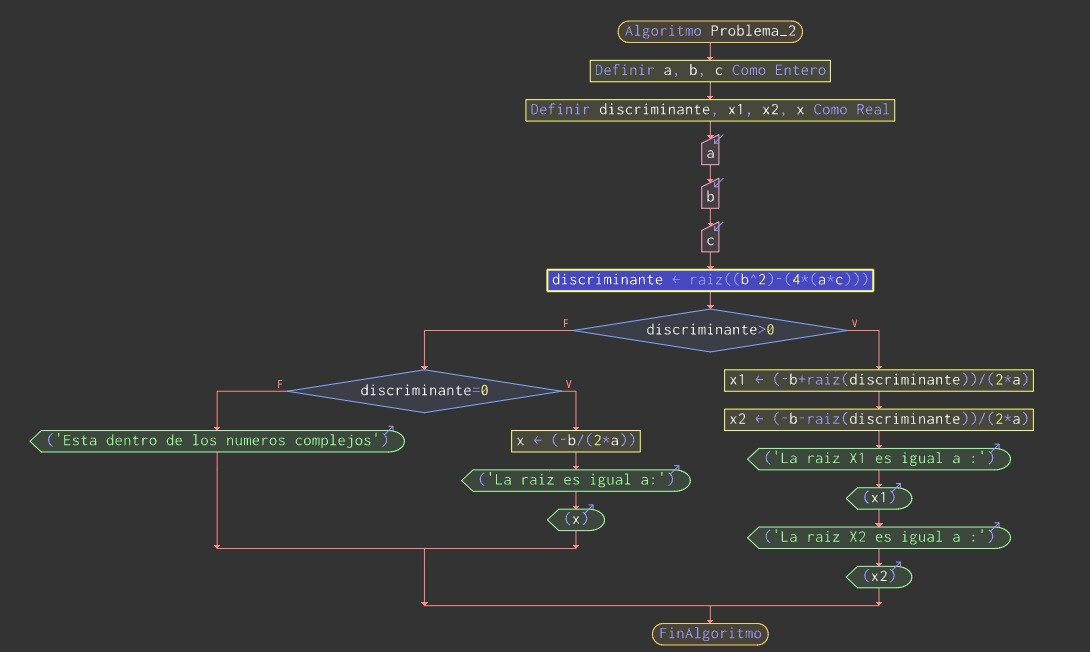
\includegraphics[width = 6 cm]{imagen/a.jpeg}
    \caption{Gráfica de la ecuación de la solución de raíces}
    \label{fig:GraficaEcuacionRecta}
\end{figure}


\section{Desarrollo del código}
La implementación del código solicita al usuario los coeficientes \(a\), \(b\), y \(c\), calcula el discriminante y aplica la lógica mencionada para determinar la naturaleza de las raíces. 
\begin{javaCode}
 Scanner in= new Scanner(System.in);
        //Solicitar los datos para la formula general.
        
        System.out.println("""
                           "Ingresa los puntos a, b, c.
                           Separadas por una coma(a, b, c): 
                           """);
        String [] datos=in.nextLine().split(",");
        //cerrar el escaneo
        in.close();
        
\end{javaCode}

Posteriormente se convierten los valores de los puntos A, B, C. en valores enteros para ser utilizados  en la formula general .

\begin{javaCode}
    //Asigna Valores de a, b, c en enteros.
        int a= Integer.parseInt(datos[0].trim());
        int b= Integer.parseInt(datos[1].trim());
        int c= Integer.parseInt(datos[2].trim());
        
\end{javaCode}
Una vez normalizados los datos, se calcula la discriminante.
\begin{javaCode}
    //Calcula la discriminante
    double discriminante=(Math.pow(b, 2)-(4*(a*c)));
\end{javaCode}

Ya que tenemos el resultado de la discriminante, dependiendo de este se realizara la operación justa, o se dirá que la discriminante esta dentro de los números complejos.\\
Si la discriminante es mayor que cero se realiza la siguiente operación y se imprimen en pantalla los 2 posibles resultados.:
\begin{javaCode}
    if (discriminante>0) {
            double x1=(-b+Math.sqrt(discriminante))/(2*a);
            
            double x2=(-b-Math.sqrt(discriminante))/(2*a);
            System.out.println("La raiz x1 es igual a " + x1);
            System.out.println("La raiz x1 es igual a " + x2);
            
        }
\end{javaCode}
En caso de que la discriminante sea igual a cero se realiza el siguiente calculo y se imprime el resultado en pantalla.:
\begin{javaCode}
    else if(discriminante==0){
            double x=(-b/(2*a));
            System.out.println("La raiz es igual a " + x);
        }
\end{javaCode}
Por ultimo, si la discriminante es menor a cero solo se imprimira en pantalla:\\"Esta dentro de los numeros complejos"
\begin{javaCode}
    else{
            System.out.println("Esta dentro de los numeros complejos");
        }
\end{javaCode}

\section{Pruebas}
\begin{center}
\begin{tabular}{|c|c|c|c|}
\hline
\textbf{\(a\)} & \textbf{\(b\)} & \textbf{\(c\)} & \textbf{\(Resultado\)} \\
\hline
1 & -3 & 2 & Raíces reales: \(x_1 = 2, x_2 = 1\) \\
\hline
1 & 2 & 1 & Raíz real única: \(x = -1\) \\
\hline
1 & -2 & 5 & Raíces complejas \\
\hline
\end{tabular}
\end{center}

\section{Conclusión}
En resumen, el programa aborda la resolución de ecuaciones cuadráticas, clasificando las raíces entre reales y complejas mediante la evaluación del discriminante, destacando la utilidad de la fórmula cuadrática en este contexto.

\newpage
Contenido del segundo problema...
\newpage


\section{Sección Problema 3}
Contenido del tercer problema...
\newpage 
Contenido del tercer problema...
\newpage 


\section{Sección Problema 4}
Contenido del cuarto problema...
\newpage 
Contenido del cuarto problema...
\newpage 


\section{Sección Problema 5}
Contenido del quinto problema...
\newpage 
Contenido del quinto problema...
\newpage 


\section{Sección Problema 6}
Contenido del sexto problema...
\newpage 
Contenido del sexto problema...
\newpage 



\end{document}

